\newcommand{\sur}[1]{\ensuremath{^{\textrm{#1}}}}
\newcommand{\sous}[1]{\ensuremath{_{\textrm{#1}}}}
\newenvironment{Snugshade}[1][236,236,236]{
  \definecolor{shadecolor}{RGB}{#1}%
  \begin{snugshade}%
}{%
    \end{snugshade}%
}
\definecolor{shadecolor}{RGB}{236,236,236} %defines color of snugshade box
\section{Overview}


This tutorial presents the general principles of assessing the reliability of a phylogenetic inference through the use
of posterior predictive simulation (PPS). PPS works by assessing the fit of an evolutionary model to a given dataset,
and analyzing several test statistics using a traditional goodness-of-fit framework to help explain where a model
may be the most inadequate. 

\subsection{Requirements}
We assume that you have read and hopefully completed the following tutorials:
\begin{itemize}
\item RB\_Getting\_Started
\item RB\_Data\_Tutorial
\item RB\_MCMC\_Tutorial
\end{itemize}
This means that we will assume that you know how to execute and load data into \RevBayes, are familiar 
with some basic commands, and know how to perform an analysis of a single-gene dataset (assuming an 
unconstrained/unrooted tree).


%%%%%%%%
%%   Data   %%
%%%%%%%%
\section{Data and files}

We provide the necessary data and scripts that we will use in this tutorial.
Of course, you may want to use your own dataset instead.
In the \cl{data} folder, you will find the following files
\begin{itemize}
\item \textbf{data/primates\_and\_galeopterus\_cytb.nex}: A simple dataset consisting of 8 taxa with 500 characters simulated under the GTR model.
\end{itemize}

%\section{Specific Style Notes For This Tutorial}
%Throughout this tutorial you will see code snippets in various boxes like this: 
%{\tt \begin{snugshade*}
%\begin{lstlisting}
%CODE SNIPPET IN FILE
%\end{lstlisting}
%\end{snugshade*}}
%
%if the snippet is in a grey box like the one above, that is code you should inspect or tweak in a \textbf{.Rev} file.
%If the code is in blue like this: 
%{\tt \begin{Snugshade}[184,207,236]
%\begin{lstlisting}
%CODE SNIPPET TO TYPE DIRECTLY INTO RevBayes
%\end{lstlisting}
%\end{Snugshade}}
%you should type this code directly into the \RevBayes prompt in your terminal window.

\section{Introduction}
Assessing the fit of an evolutionary model to the data is critical as using a model with poor fit can lead to 
spurious conclusions. However, a critical evaluation of absolute model fit is rare in evolutionary studies.
Posterior prediction is a Bayesian approach to assess the fit of a model to a given dataset \citep{Bollback2002-ki,Brown2014-jl,Gelman2014-ay},
that relies on the use of the posterior and the posterior predictive distributions. 
The posterior distribution is the standard output from Bayeisan phylogenetic inference. The posterior predictive 
distribution represents a range of possible outcomes given the assumptions of the model. The most common method to 
generate these possible outcomes, is to sample parameters from the posterior distribution, and use them 
to simulate new replicate datasets (Fig. 1). If these simulated datasets differ from the empirical dataset in a
meaningful way, the model is failing to capture some salient feature of the evolutionary process. 

\begin{figure}[t!]
\centering
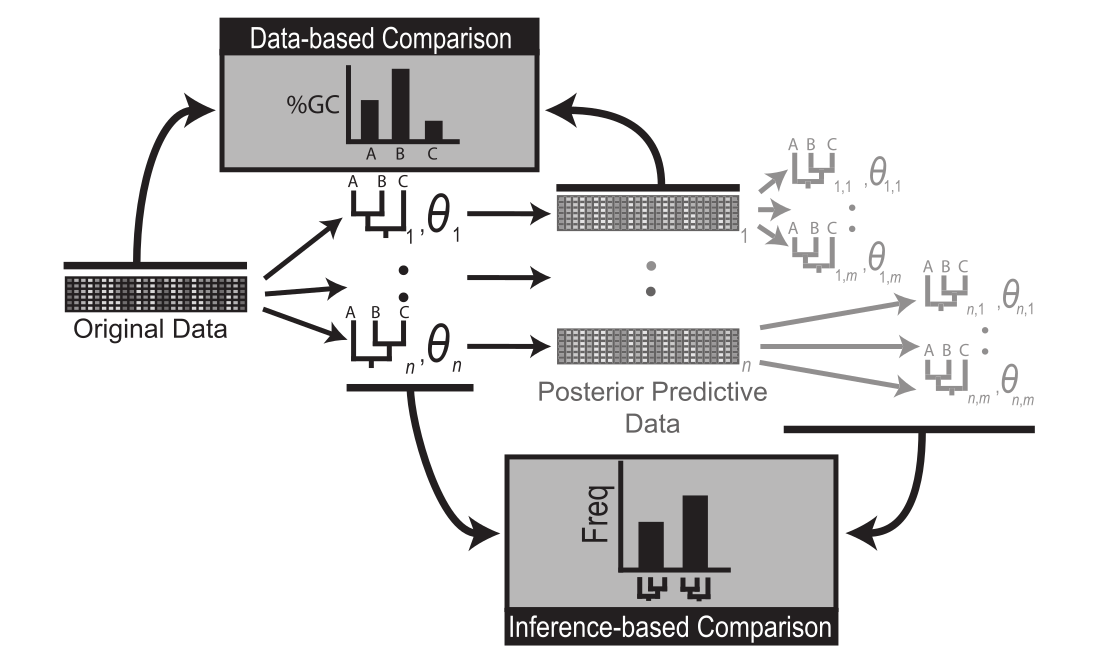
\includegraphics[width=\textwidth,angle=0]{figures/brown_2014.png}
\caption{\small 
    %A cartoon schematic showing the process of assessing model fit with posterior predictive simulation built into P\sur{3} and \RevBayes. \label{"Figure 1"}}
A schematic representation of data- versus inference-based approaches to assessing model plausibility with posterior predictive
simulation. Most statistics proposed for testing model plausibility compare data-based characteristics of the original data set to the posterior
    predictive data sets (e.g., variation in GC-content across species). 
    \RevBayes additionally implements test statistics that compare the inferences
    resulting from different data sets (e.g., the distribution of posterior probability across topologies). Multiple sequence alignments (MSAs) are
    represented as shaded matrices and arrows originating from MSAs point to the MCMC samples of tree topologies and scalar model parameters
    ($\theta$) resulting from Bayesian analysis of that MSA. Subscripts of MCMC samples taken during analysis of the original data index the samples $(1,
    ..., n)$. Subscripts for each posterior predictive data set indicate which MCMC sample was used in its simulation. Subscripts for MCMC samples
    resulting from analysis of a posterior predictive data set first indicate the posterior predictive data set that was analyzed and next index the
    MCMC samples from analysis of that particular data set $(1, ..., m)$.
    \label{"Figure 1"}}
%\end{centering}
\end{figure}
The framework to construct posterior predictive distributions, and compare them to the posterior distribution is 
conveniently built in to \RevBayes. In this tutorial we will walk you through using this functionality to perform
a complete posterior predictive simulation on an example dataset.  

\subsection{Data- Versus Inference-Based Comparisons}

Most statistics proposed for testing model plausibility compare data-based characteristics of the original data set to the posterior
    predictive data sets (e.g., variation in GC-content across species).
    In data-based assessments of model fit one compares the empirical data to data simulated from samples of the posterior distribution.
    \RevBayes additionally implements test statistics that compare the inferences
        resulting from different data sets (e.g., the distribution of posterior probability across topologies).
        These are called inference-based assessments of model fit. For these assessments one must run an MCMC analysis
        on each simulated data set, and then compare the inferences made from the simulated data to the inference made from the empirical data.

Due to time constraints, in today's tutorial we will only cover the data-based method of assessing model plausibility. 
The inference-based method can be a powerful tool that you may want to explore at another time.

\bigskip
\subsection{Substitution Models}\label{secUnif} 

The models we use here are equivalent to the models described in the previous exercise on substitution models (continuous time Markov models).
To specify the model please consult the previous exercise. Specifically, you will need to specify the following substitution models:
\begin{itemize}
\item Jukes-Cantor (JC) substitution model \citep{Jukes1969-jp}
\item General-Time-Reversible (GTR) substitution model \citep{Tavare1986-ij}
\item Gamma (+G) model for among-site rate variation \citep{Yang1994-ep}
\item Invariable-sites (+I) model \citep{Hasegawa1985-ir}
\end{itemize}


\bigskip
\section{Assessing Model Fit with Posterior Prediction}

The entire process of posterior prediction can be executed by using the \textbf{data\_pp\_analysis\_JC.Rev} script in the \textbf{scripts}
folder. If you were to type the following command into \RevBayes:

{\tt \begin{Snugshade}[184,207,236]
\begin{lstlisting}
source("scripts/data_pp_analysis_JC.Rev")
\end{lstlisting}
\end{Snugshade}}

the entire data-based posterior prediction process would run on the example dataset. However, in this tutorial, we 
will walk through each step of this process on an example dataset. 

\subsection{Empirical MCMC Analysis}

To begin, we first need to generate a posterior distribution from which to sample for simulation. 
This is the normal, and often only, step conducted in phylogenetic studies. Here we will specify our 
dataset, evolutionary model, and run a traditional MCMC analysis. 

This code is all in the \textbf{data\_pp\_analysis\_JC.Rev} file.

\subsubsection{Set up the workspace}

First, let's set up some workspace variables we'll need.
We'll specify a general name to apply to your analysis. This will be used for future output files, so make sure it's something clear and easy to understand.
{\tt \begin{Snugshade}[184,207,236]
\begin{lstlisting}
analysis_name = "pps_example"
model_name = "JC"
model_file_name = "scripts/"+model_name+"_Model.Rev"
\end{lstlisting}
\end{Snugshade}}

Now specify and read in the input file. This is your sequence alignment in NEXUS format.
{\tt \begin{Snugshade}[184,207,236]
\begin{lstlisting}
in_file = "data/primates_and_galeopterus_cytb.nex"
data <- readDiscreteCharacterData(in_file)
\end{lstlisting}
\end{Snugshade}}

\subsubsection{Specify the model}

Now we'll call a separate script \textbf{JC\_Model.Rev} that specifies the JC model:
{\tt \begin{Snugshade}[184,207,236]
\begin{lstlisting}
source( model_file_name ) 
\end{lstlisting}
\end{Snugshade}}

If we open the \textbf{JC\_Model.Rev} 
script, most of this script should look familiar from the RB\_MCMC\_Tutorial. There are a couple of specific 
lines we can look at that might be a little different though, as we are using a unrooted tree for this
analysis. 

{\tt \begin{Snugshade}[184,207,236]
\begin{lstlisting}
Q <-fnJC(4)
\end{lstlisting}
\end{Snugshade}}

Here we are specifying that we should use the Jukes-Cantor model, and have it applied uniformly to all sites in 
the dataset. While this obviously is not likely to be a good fitting model for most datasets, we are using it for 
simplicity of illustrating the process. 

{\tt \begin{Snugshade}[184,207,236]
\begin{lstlisting}
topology ~ dnUniformTopology(names)
\end{lstlisting}
\end{Snugshade}}
This sets a uniform prior on the tree topology.
{\tt \begin{Snugshade}[184,207,236]
\begin{lstlisting}
br_lens[i] ~ dnExponential(10.0)
\end{lstlisting}
\end{Snugshade}}
This sets an exponential distribution as the branch length prior.
{\tt \begin{Snugshade}[184,207,236]
\begin{lstlisting}
phylogeny := treeAssembly(topology, br_lens)
\end{lstlisting}
\end{Snugshade}}
This builds the tree by combining the topology with branch length support values.

\subsubsection{Run the MCMC}

Now let's run MCMC on our empirical dataset, just like
a normal phylogenetic analysis. Here we use the Jukes-Cantor
substition model.
{\tt \begin{Snugshade}[184,207,236]
\begin{lstlisting}
mcmc_gen = 10000
burnin_gen = 2000
source("scripts/MCMC_Empirical.Rev")
\end{lstlisting}
\end{Snugshade}}


After specifying a model, we will conduct the MCMC analysis with the script  \textbf{MCMC\_Empirical.Rev}. 
Much of that script should look familiar from the \textbf{RB\_CTMC\_Tutorial}, but let's take a look at 
the script and break down and revisit some of the major pieces as a refresher. Much of this will be a 
familiar to you from the \textbf{RB\_CTMC\_Tutorial}. 


First we need to specify some monitors. 
{\tt \begin{Snugshade}[184,207,236]
\begin{lstlisting}
mni = 0
monitors[++mni] = mnModel(filename="output" + n + "/" + analysis_name + "_posterior.log",printgen=2500, separator = TAB)
\end{lstlisting}
\end{Snugshade}}
{\tt \begin{Snugshade}[184,207,236]
\begin{lstlisting}
monitors[++mni] = mnFile(filename="output" + n + "/" + analysis_name + "_posterior.trees",printgen=2500, separator = TAB, phylogeny)
\end{lstlisting}
\end{Snugshade}}
{\tt \begin{Snugshade}[184,207,236]
\begin{lstlisting}
monitors[++mni] = mnScreen(printgen=2500, TL)
\end{lstlisting}
\end{Snugshade}}
{\tt \begin{Snugshade}[184,207,236]
\begin{lstlisting}
monitors[++mni] = mnStochasticVariable(filename="output" + n + "/" + analysis_name + "_posterior.var",printgen=2500)
\end{lstlisting}
\end{Snugshade}}

Here the monitors are just being advanced by the value of mni which is being incremented each generation.

Next, we will call the MCMC function, passing it the model, monitors and moves we specified above to set 
to build our mymcmc object.
 
{\tt \begin{Snugshade}[184,207,236]
\begin{lstlisting}
mymcmc = mcmc(mymodel, monitors, moves, nruns=2)
\end{lstlisting}
\end{Snugshade}}

Specify a burnin for this run.

{\tt \begin{Snugshade}[184,207,236]
\begin{lstlisting}
mymcmc.burnin(generations=burnin_gen,tuningInterval=100)
\end{lstlisting}
\end{Snugshade}}

Finally, we will execute the run for a specified number of generations. Here we are only using a small
number of generations for the tutorial, however with empirical data you will most likely need a much
larger number of generations to get a well mixed sample. The number of generations and printed generations
is important to consider here for a variety of reasons, in particular for posterior predictive simulation.
When we simulate datasets in the next step, we can only simulate 1 dataset per sample in our posterior. So,
while the number of posterior samples will almost always be larger than the number of datasets we will want
to simulate, it's something to keep in mind.


Now let's actually run the MCMC in \RevBayes. 
This process should take approximately 15-20 minutes depending on the speed of your computer.

{\tt \begin{Snugshade}[184,207,236]
\begin{lstlisting}
mymcmc.run(generations=mcmc_gen)
\end{lstlisting}
\end{Snugshade}}

\subsubsection{MCMC output}

After the process completes, the results can be found in the \textbf{output\_JC} folder. You should see a 
number of familiar looking files, all with the name we provided under the \textbf{analysis\_name} variable, 
\textbf{pps\_example} in this case. Since we set the number of runs (nruns=2) in our MCMC, there will be two files 
of each type (.log .trees .var) with an \_\textit{N} where \textit{N} is the run number. You will also see 3 files without 
any number in their name. These are the combined files of the output. These will be the files we use for 
the rest of the process. If you open up one of the combined .var file, you should see that there are 200 
samples. This was produced by our number of generations (250,000) divided by our number of printed generations,
(2500) what we specified earlier. This is important to note, as we will need to thin these samples 
appropriately in the next step to get the proper number of simulated datasets. 


\subsection{Posterior Predictive Data Simulation}
The next step of posterior predictive simulation is to simulate new datasets by drawing samples and 
parameters from the posterior distribution generated from the empirical MCMC anlaysis. 

In the \textbf{data\_pp\_analysis\_JC.Rev} script, that is conducted using the following lines of RevScript: 
{\tt \begin{Snugshade}[184,207,236]
\begin{lstlisting}
source("scripts/PosteriorPredictive_Simulation.Rev")
\end{lstlisting}
\end{Snugshade}}

Let's take a look at each of the calls in the \textbf{PosteriorPredictive\_Simulation.Rev} script so 
that we can understand what is occurring. 

First, we read in the trace file of the Posterior Distribution of Variables.
{\tt \begin{Snugshade}[184,207,236]
\begin{lstlisting}
trace = readStochasticVariableTrace("output" + "/" + analysis_name + "_posterior.var", delimiter=TAB)
\end{lstlisting}
\end{Snugshade}}

Now we call the \textbf{posteriorPredictiveSimulation()} function, which accepts any valid model of sequence evolution, and output directory, and a trace. For each line in the trace, it will simulate a new dataset under the specified model.
{\tt \begin{Snugshade}[184,207,236]
\begin{lstlisting}
pps = posteriorPredictiveSimulation(mymodel, directory="output" + "/" + analysis_name + "_post_sims", trace)
\end{lstlisting}
\end{Snugshade}}

Now we run the posterior predictive simulation, generating a new dataset for each line in the trace file 
that was read in. This is the part where we need to decide how many simulated datasets we want to generate.
If we just use the pps.run() command, one dataset will be generated for each sample in our posterior distribution.
In this case, since we are reading in the combined posterior trace file with 200 
samples, it would generate 200 simulated datasets. If you want to generate fewer, say 100 datasets,
you need to use the thinning argument as above. In this case, we are thinning the output by 2, that is
we are dividing our number of samples by 2. So that in our example case, we will end up simulating 100 
new datasets.
{\tt \begin{Snugshade}[184,207,236]
\begin{lstlisting}
pps.run(thinning=2)
\end{lstlisting}
\end{Snugshade}}


This process should finish in just a minute or two. If you look in the \textbf{output\_JC} folder, there should be 
another folder called \textbf{pps\_example\_post\_sims}. This folder is where the simulated datasets are saved. 
If you open it up, you should see 100 folders named posterior\_predictive\_sim\_\textit{N}. Where \textit{N} 
is the number of the simulated dataset. In each of these folders, you should find a seq.nex file. If you 
open one of those files, you'll see it's just a basic NEXUS file. These will be the datasets we analyze 
in the next step.


\subsection{Calculating the Test Statistics}

Now we will calculate the test statistics from the 
empirical data and the simulated data sets. The part in the \textbf{data\_pp\_analysis\_JC.Rev}
script that generates the test statistics is the following line:

{\tt \begin{Snugshade}[184,207,236]
\begin{lstlisting}
num_post_sims = listFiles(path="output_"+model_name+"/" + analysis_name + "_post_sims").size()
source("scripts/PosteriorPredictive_DataSummary.Rev")
\end{lstlisting}
\end{Snugshade}}


We will look at the 
major concepts of the \textbf{PosteriorPredictive\_DataSummary.Rev} to better understand how it works. For a more complete discussion of the 
statistics involved, please review \cite{Brown2014-mb, Doyle2015-qb}. In general, this script and these 
statistics work by calculating the statistics of interest across each posterior distribution from the 
simulated datasets, and comparing those values to the values from the empirical posterior distribution.

The current version of this script generates over 30 summary statistics including: 
\begin{itemize}
\item Number Invariant Sites
\item Max Pairwise Difference
\item Max GC Content
\item Min GC Content
\item Mean GC Content
\end{itemize}

There are functions built-in to \RevBayes to calculate these values for you. Here are some examples
from the \textbf{PosteriorPredictive\_DataSummary.Rev} script: 

{\tt \begin{Snugshade}[184,207,236]
\begin{lstlisting}
max_pd          = sim_data.maxPairwiseDifference( excludeAmbiguous=FALSE )
mean_gc_1       = sim_data.meanGcContentByCodonPosition(1, excludeAmbiguous=FALSE )
var_gc_1        = sim_data.varGcContentByCodonPosition(1, excludeAmbiguous=FALSE )
\end{lstlisting}
\end{Snugshade}}

\smallbreak
These same statistics are calculated for both the posterior distributions from the simulated datasets
and the posterior distribution from the empirical dataset.

\subsection{Calculating \textit{P}-values and effect sizes}

Once we have the test statistics calculated for the simulated and empirical posterior distributions, 
we can compare the simulated to the empirical to get a goodness-of-fit. One simple way to do this is to calculate a posterior 
predictive \textit{P}\-value for each of the test statistics of interest. This is done in the \textbf{data\_pp\_analysis\_JC.Rev} with the following lines :

{\tt \begin{Snugshade}[184,207,236]
\begin{lstlisting}
emp_pps_file = "results_" + model_name + "/empirical_data_" + analysis_name + ".tsv"
sim_pps_file = "results_" + model_name + "/simulated_data_" + analysis_name + ".tsv"
outfileName = "results_" + model_name + "/data_pvalues_effectsizes_" + analysis_name + ".tsv"
source("scripts/PosteriorPredictive_PValues.Rev")
\end{lstlisting}
\end{Snugshade}}

The 3 posterior predictive \textit{P}\-values currently
calculated by \RevBayes are: 

\begin{itemize}
\item Lower 1-tailed 
\item Upper 1-tailed
\item 2-tailed
\end{itemize}

The posterior predictive \textit{P}\-value for a lower one-tailed test is the proportion of samples in the distribution
where the value is less than or equal to the observed value, calculated as:

\begin{equation*} 
    p_l=p(T(X_{rep})\leqslant T(X)|(X)
\end{equation*}

The posterior predictive \textit{P}\-value for a lower one-tailed test is the proportion of samples in the distribution
where the value is greater than or equal to the observed value, calculated as:

\begin{equation*} 
    p_u=p(T(X_{rep})\geqslant T(X)|(X)
\end{equation*}

and the two-tailed posterior predictive \textit{P}\-value is simply twice the minimum of the corresponding one-tailed tests
calculated as:

\begin{equation*} 
p_2=2min(p_l,p_u)
\end{equation*}

Let's take a look at the \textbf{PosteriorPredictive\_PValues.Rev} script to get a better idea of what is 
happening.

Using the equations outlined above, this script reads in the simulated and empirical data we just calculated, and calls a few simple functions
for each of the test statistics:

{\tt \begin{Snugshade}[184,207,236]
\begin{lstlisting}
## Calculate and return a vector of lower, equal, and upper pvalues for a given test statistic
p_values <- posteriorPredictiveProbability(numbers, empValue)

## 1-tailed
lower_p_value <- p_values[1] 
equal_p_value <- p_values[2] 
upper_p_value <- p_values[3] 

## mid-point
midpoint_p_value = lower_p_value + 0.5*equal_p_value

## 2-tailed
two_tail_p_value = 2 * (min(v(lower_p_value, upper_p_value)))
\end{lstlisting}
\end{Snugshade}}

these snippets calculate the various p-values of interest to serve as our goodness-of-fit test. 


Another way that you can calculate the magnitude of the discrepancy between the empirical and PP datasets is by
calculating the effect size of each test statistic. Effect sizes are useful in quantifying the magnitude of the difference between the 
empirical value and the distribution of posterior predictive values. The test statistic effect size can be calculated by taking the 
absolute value of the difference between the median posterior predictive value and the empirical value divided by 
the standard deviation of the posterior predictive distribution \citep{Doyle2015-qb}. Effect sizes are calculated automatically for the inference based test statistics in the P\sur{3} analysis. The effect sizes for each test statistics are stored in the same output file as the \textit{P}\-values. 

{\tt \begin{Snugshade}[184,207,236]
\begin{lstlisting}
effect_size = abs((m - empValue) / stdev(numbers))
\end{lstlisting}
\end{Snugshade}}


calculates the effect size of a given test statistic. 


\subsection{Viewing the Results}

Once execution of the script is complete, you should see a new directory, names \textbf{results\_JC}. In this folder there should be 3 files. Each of these is a simple tab-delimited (TSV) file containing the test statistic calculation output.

\begin{itemize}
\item empirical\_pps\_example.tsv
\item pps\_example.tsv
\item pvalues\_pps\_example.tsv
\end{itemize}

If you have these 3 files, and there are results in them, you can go ahead and quit \RevBayes.

{\tt \begin{Snugshade}[184,207,236]
\begin{lstlisting}  
q()
\end{lstlisting}
\end{Snugshade}}

\begin{figure}[!t]
\centering
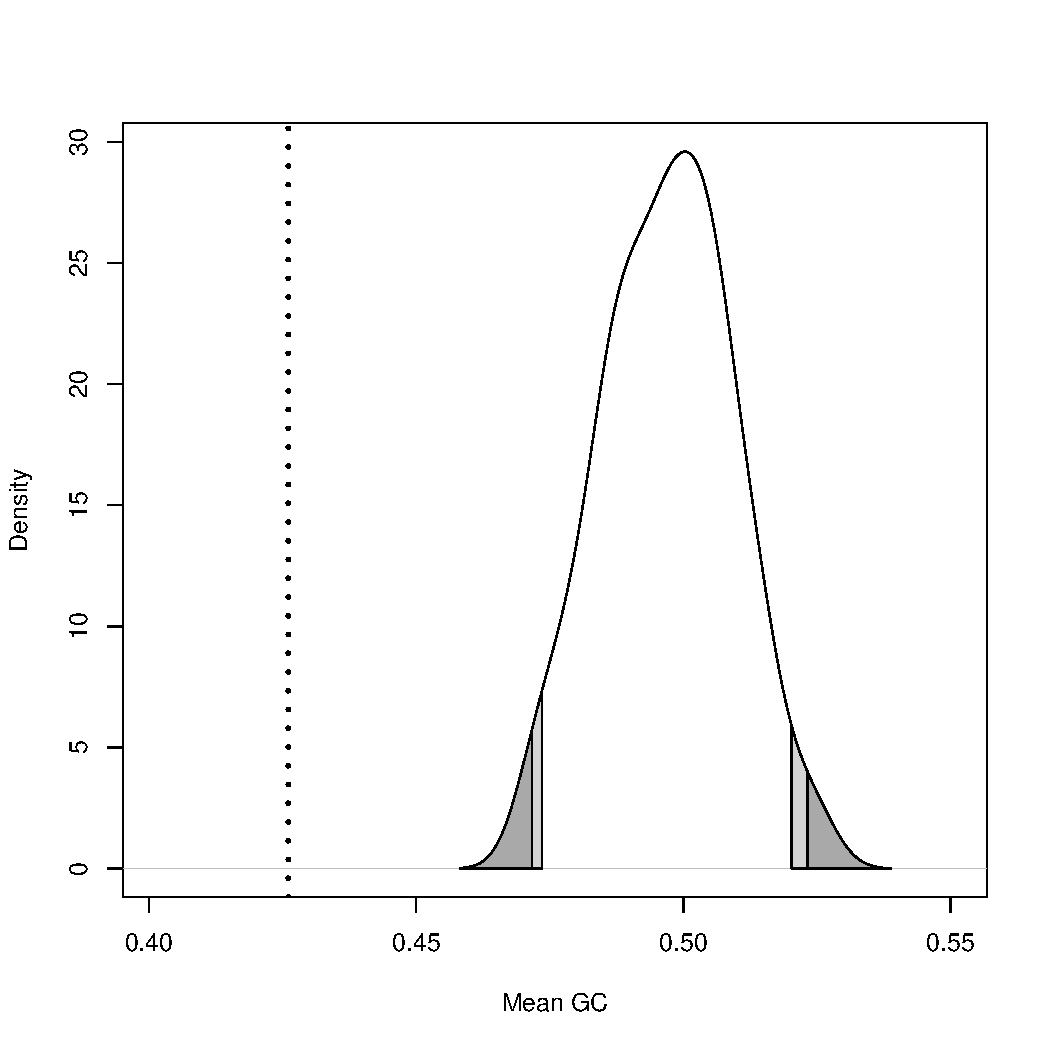
\includegraphics[width=\textwidth,angle=0]{figures/mean_gc.pdf}
\caption{\small 
The distribution of mean GC values calculated from the simulated data sets
is shown. The dotted line represents the mean GC calculated from the empirical data set.
The Jukes-Cantor model does not adequately describe the empirical data.
    This plot was generated in \R using the \textbf{scripts/plot\_results.R} script.
    }
\end{figure}

You can get an estimate of how the model performed by examining the \textit{P}\-values in the 
\textbf{inference\_pvalues\_effectsizes\_pps\_example.csv} and \textbf{data\_pvalues\_effectsizes\_pps\_example.csv} files. In this example, a quick view shows us that most of the statistics show a value less than 0.05. This leads to a rejection of the model, suggesting 
that the model employed is not a good fit for the data. This is the result we expected given we chose a very 
simplistic model (JC) that would likely be a poor fit for our data. However, it's a good example 
of the sensitivity of this method, showing how relatively short runtimes and a low number of generations will 
still detect poor fit. 


You can also use \R to plot the results. Run the \R script \textbf{scripts/plot\_results.R}.
This will generate a pdf plot for every test statistic.




\subsection{Additional Exercises}

Included in the \textbf{scripts} folder is a second model script called \textbf{GTR\_Model.Rev}. 
As a personal exercise and a good test case, take some time now, and run the same analysis, substituting
the \textbf{GTR\_Model.Rev} model script for the \textbf{JC\_Model.Rev} script we used in the earlier example.
You should get different results, this is an excellent chance to explore the results and think about what
they suggest about the fit of the specified model to the dataset. 

\subsubsection{Additional Exercises}
\textbf{Some Questions to Keep in Mind:}
\begin{itemize}
  \item Do you find the goodness-of-fit results to suggest that the GTR or JC model is a better fit for our data? 
  \item Which test statistics seem to show the strongest effect from the use of a poorly fitting model?
  \item Other than \textit{P}\-values, what other ways might you explore the test statistic distributions to identify poor fit?
\end{itemize}


\newpage
\section{For your consideration...}
In this tutorial you have learned how to use \RevBayes to assess the fit of a substitution model 
to a given sequence alignment. As you have discovered, the observed data should be plausible under 
the posterior predictive simulation if the model is reasonable. In phylogenetic analyses we choose a model, which explicitly assumes 
that it provides an reasonable explanation of the evolutionary process that generated our data. However, 
just because a model may be the 'best' model available, does not mean it is an appropriate model for the data. 
This distinction becomes both more critical and less obvious in modern analyses, where the 
number of genes often number in the thousands. Posterior predictive simulation in \RevBayes, allows you
to easily check model fit for a large number of genes by using global summaries to check the posterior 
predictive distributions with a comfortable goodness-of-fit style framework. 

\subsection{Batch Processing of Large Datasets}
The process described above is for a single gene or alignment. However, batch processing a large number of genes
with this method is a relatively straight forward process. 

\RevBayes has built in support for MPI so running \RevBayes on more than a single processor, or on a cluster is 
as easy as calling it with openmpi. 

For example:
{\tt \begin{snugshade*}
\begin{lstlisting}
mpirun -np 16 rb-mpi scripts/full_analysis.Rev
\end{lstlisting}
\end{snugshade*}}
would run the entire posterior predictive simulation analysis on a single dataset using 16 processors
instead of a single processor. Use of the MPI version of \RevBayes will speed up the process dramatically.

Setting up the \textbf{full\_analysis.Rev} script to cycle through a large number of alignments is relatively
simple as well. One easy way is to provide a list of the data file names, and to loop through 
them. As an example:

{\tt \begin{snugshade*}
\begin{lstlisting} 
data_file_list = "data_file_list.txt" 
data_file_list <- readDiscreteCharacterData(data_file_list)
file_count = 0

for (n in 1:data_file_list.size()) {

FULL_ANALYSIS SCRIPT GOES HERE

file_count = file_count + 1
}
\end{lstlisting}
\end{snugshade*}}

Then, anywhere in the full\_analysis portion of the script that the lines
{\tt \begin{snugshade*}
\begin{lstlisting} 
inFile = "data/8taxa_500chars_GTR.nex"
analysis_name = "pps_example"
\end{lstlisting}
\end{snugshade*}}
appear, you would replace them with something along the lines of: 
{\tt \begin{snugshade*}
\begin{lstlisting} 
inFile = n
analysis_name = "pps_example_" + file_count
\end{lstlisting}
\end{snugshade*}}

This should loop through all of the data files in the list provided, and run the full posterior predictive
simulation analysis on each file. Using a method like this, and combining it with the MPI call above, you can scale
this process up to multiple genes and spread the computational time across several cores to speed it up. 

\bigskip
\bibliographystyle{sysbio}
\bibliography{pps}
